\documentclass{standalone}
\usepackage{amssymb} %for Blackboard bold etc
\usepackage{amsmath}
\usepackage{amsfonts}
\usepackage{tikz}
\usetikzlibrary{calc,3d,arrows,shapes}
\usepackage{tikz-3dplot}
\usetikzlibrary{decorations.shapes}
\usetikzlibrary{arrows,shapes,positioning}

\usetikzlibrary{external}%%%
\tikzexternalize % activate!
\definecolor{ligthgray}{rgb}{0.9,0.9,0.9}
\definecolor{ligthblue}{rgb}{0.529411764705882,0.807843137254902,0.9215}

\begin{document}


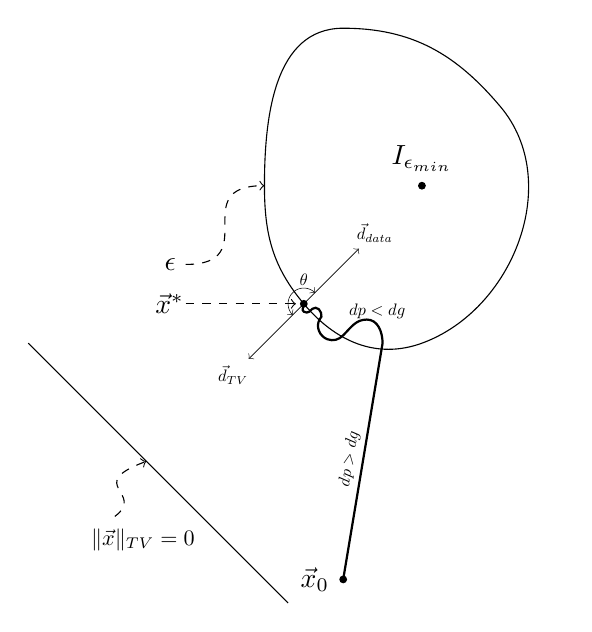
\begin{tikzpicture}

\draw (4,4) node[circle,fill,inner sep=1pt,label=above:$I_{\epsilon_{min}}$]{};

\draw [thin](2,4)to[out=90,in=-180] (3,6)to[out=0,in=130] (5,5)to[out=-50,in=20](4,2)to[out=-160,in=-50](2.5,2.5)to[out=130,in=-90](2,4);


%\draw (0,0) node[circle,fill,inner sep=1pt,label=above:$I_{TV_{min}}$]{};
%\draw (-1,0)to[out=90,in=-180] (0,2)to[out=0,in=100] (1,1)to[out=-80,in=20](0,-2)to[out=-160,in=-90](-1,0);

\node[anchor=east] at (1,3){$\epsilon$};
\draw[->,dashed](1,3).. controls ([xshift=1cm] 1,3) and ([xshift=-1cm] 2,4) .. (2,4);

\node[anchor=east] at (1.1,2.5){$\vec{x}^*$};

\draw[->,dashed](1,2.5)-- (2.4,2.5);



\draw (3,-1) node[circle,fill,inner sep=1pt,label=left:$\vec{x}_0$]{};

\draw[thick] (3,-1)--(3.5,2)node[midway,above,sloped,scale=0.6]{$dp>dg$} to[out=90,in=0](3.3,2.3)to[out=180,in=45](3,2.1)to[out=180+45,in=-20](2.8,2.05) to [out=160,in=180+60](2.7,2.3)to[out=30,in=0](2.65,2.45)to[out=180,in=45](2.57,2.4)to[out=180+45,in=-20](2.5,2.4)to[out=150,in=-90](2.5,2.5);

\node[scale=0.6,anchor=west]at(3,2.4){$dp<dg$};


\draw (2.5,2.5) node[circle,fill,inner sep=1pt]{};

\draw[->,very thin](2.5,2.5)--(3.2,3.2);\node[scale=0.6] at(3.4,3.4){$\vec{d}_{data}$};
\draw[->,very thin](2.5,2.5)--(1.8,1.8);\node[scale=0.6] at(1.6,1.6){$\vec{d}_{TV}$};

   \draw [<->,black,very thin,domain=45:225] plot ({0.2*cos(\x)+2.5}, {0.2*sin(\x)+2.5});
   \node[scale=0.6] at(2.5,2.8){$\theta$};
   
   \draw[thin](2.3,-1.3)--(-1,2);
   \node[anchor=west,scale=0.8]at(-0.3,-0.5){$\lVert \vec{x}\rVert_{TV}=0$};
   
   \draw[->,dashed](0.1,-0.2).. controls ([xshift=0.5cm] 0,0.1) and ([xshift=-0.5cm] 0.2,0.2) .. (0.5,0.5);

\end{tikzpicture}



\end{document}